% thoughts:
% - we introduce fork/join as simply creating threads to divide the work and then combining the results, without any recursion. but that is not a parallel algo. parallel DnC is though. Maybe we should introduce it as intrinsically recursive. the paper introduces fork/join as parallel versions of DnC.
% - we say that the joining is combining results. is it? is it not the waiting for them to finish? framework suggests it is.
% - maybe change the figure of DnC to F/J
%


% - is the argument of forkjoinpool really the max amount
% of threads?
% - do I have to shutdown the fjpool?
% - write comment about the code in fork join
% - two tricks with cutoff and compute. maybe show them already when we are using threads, else the reader might ask itself
% - write about cilk


\documentclass[main.tex]{subfiles}
\setlength{\columnsep}{3cm}
\setcounter{secnumdepth}{3}
\begin{document}

\addtolength{\tabcolsep}{-2pt}

\section{Parallel Algorithms}
In the previous chapter, we discussed how \textit{Amdahl's Law} tells us how our programs are inherently bottlenecked by their non-parallelizable part, no matter how many processor we have available. Hence, it is our goal to reduce the sequential fraction of our programs when we want to run them on many processors. To this end, we introduce some parallel algorithms in this chapter. Here, parallelization means that we divide up the task at hand onto different \textit{threads}, assuming that they are able to run on different \textit{processors}. This is in contrast to Chapter 3, where we assumed a fixed program that will be run on a single processor (imagine this is the work chunk a thread was assigned to process) and analyzed how we can exploit independence within this set of instructions.\\
We can use the techniques learned in this chapter to design parallel implementations of algorithms.

\subsection{Fork-Join Parallelism}
Let us once again consider the task of summing up an array. Using task parallelism, we can simply divide up the array on some number of threads. Each thread sums up some part of the array and finally, the main thread sums up these partial results. The corresponding code looks something like this in Java:
\begin{figure}[H]
    \begin{minted}[]{java}
int sum(int[] arr) { // can be a static method
    int len = arr.length;
    int ans = 0;
    SumThread[] ts = new SumThread[4];
    for (int i = 0; i < 4; i++) { // do parallel computations
        ts[i] = new SumThread(arr, i*len/4, (i+1)*len/4);
        ts[i].start();
    }
    for (int i=0; i < 4; i++) { // combine results
        ts[i].join(); // wait for helper to finish!
        ans += ts[i].ans;
    }
    return ans;
}
    \end{minted}
\end{figure}
\noindent Here, \texttt{SumThread} is some \texttt{Thread} class summing up the given indices. We do not really care about its exact implementation here.\\[3mm]
This approach of dividing up the work into multiple different tasks and then combining their results is called \textit{Fork-Join Parallelism}. The join here does not refer to the \texttt{Thread.join()} method, where we wait for a thread to finish, but to the combining of partial results (in this case the main threads sums up the partial results).

\subsubsection{Parallel Divide-And-Conquer}
Above solution is not new to us. But we will improve upon it. Assume we want to run above code on some hardware efficiently. We find a few things that are not optimal with this general approach:
\begin{itemize}
  \item There is a fixed number of threads created (four in this case), no matter how many processors the underlying hardware has. We can solve this by making the number of threads created a parameter of the method.
  \item For general datastructures, dividing it into equal chunks for threads to process can lead to large workload imbalances across threads. Consider a graph datastructure. When we give the same number of vertices to each thread to process, the number of edges in a vertex set might be vastly different. When we now want to run parallel BFS, we will not get good speedup, because the few threads with the most edges will bottleneck the runtime. In this case, this is not a problem, since each thread will have about the same workload with summing array entries.
  \item We have a sequential bottleneck of summing up the partial results in the end.
\end{itemize}
We can improve on the last point by parallelizing the result combination. This can easily be implemented by recursively dividing the tasks with the Fork-Join model. This gives us a parallel version of the \textit{divide-and-conquer} paradigm. The basic structure of a divide-and-conquer program is the following:
\begin{figure}[H]
    \centering
    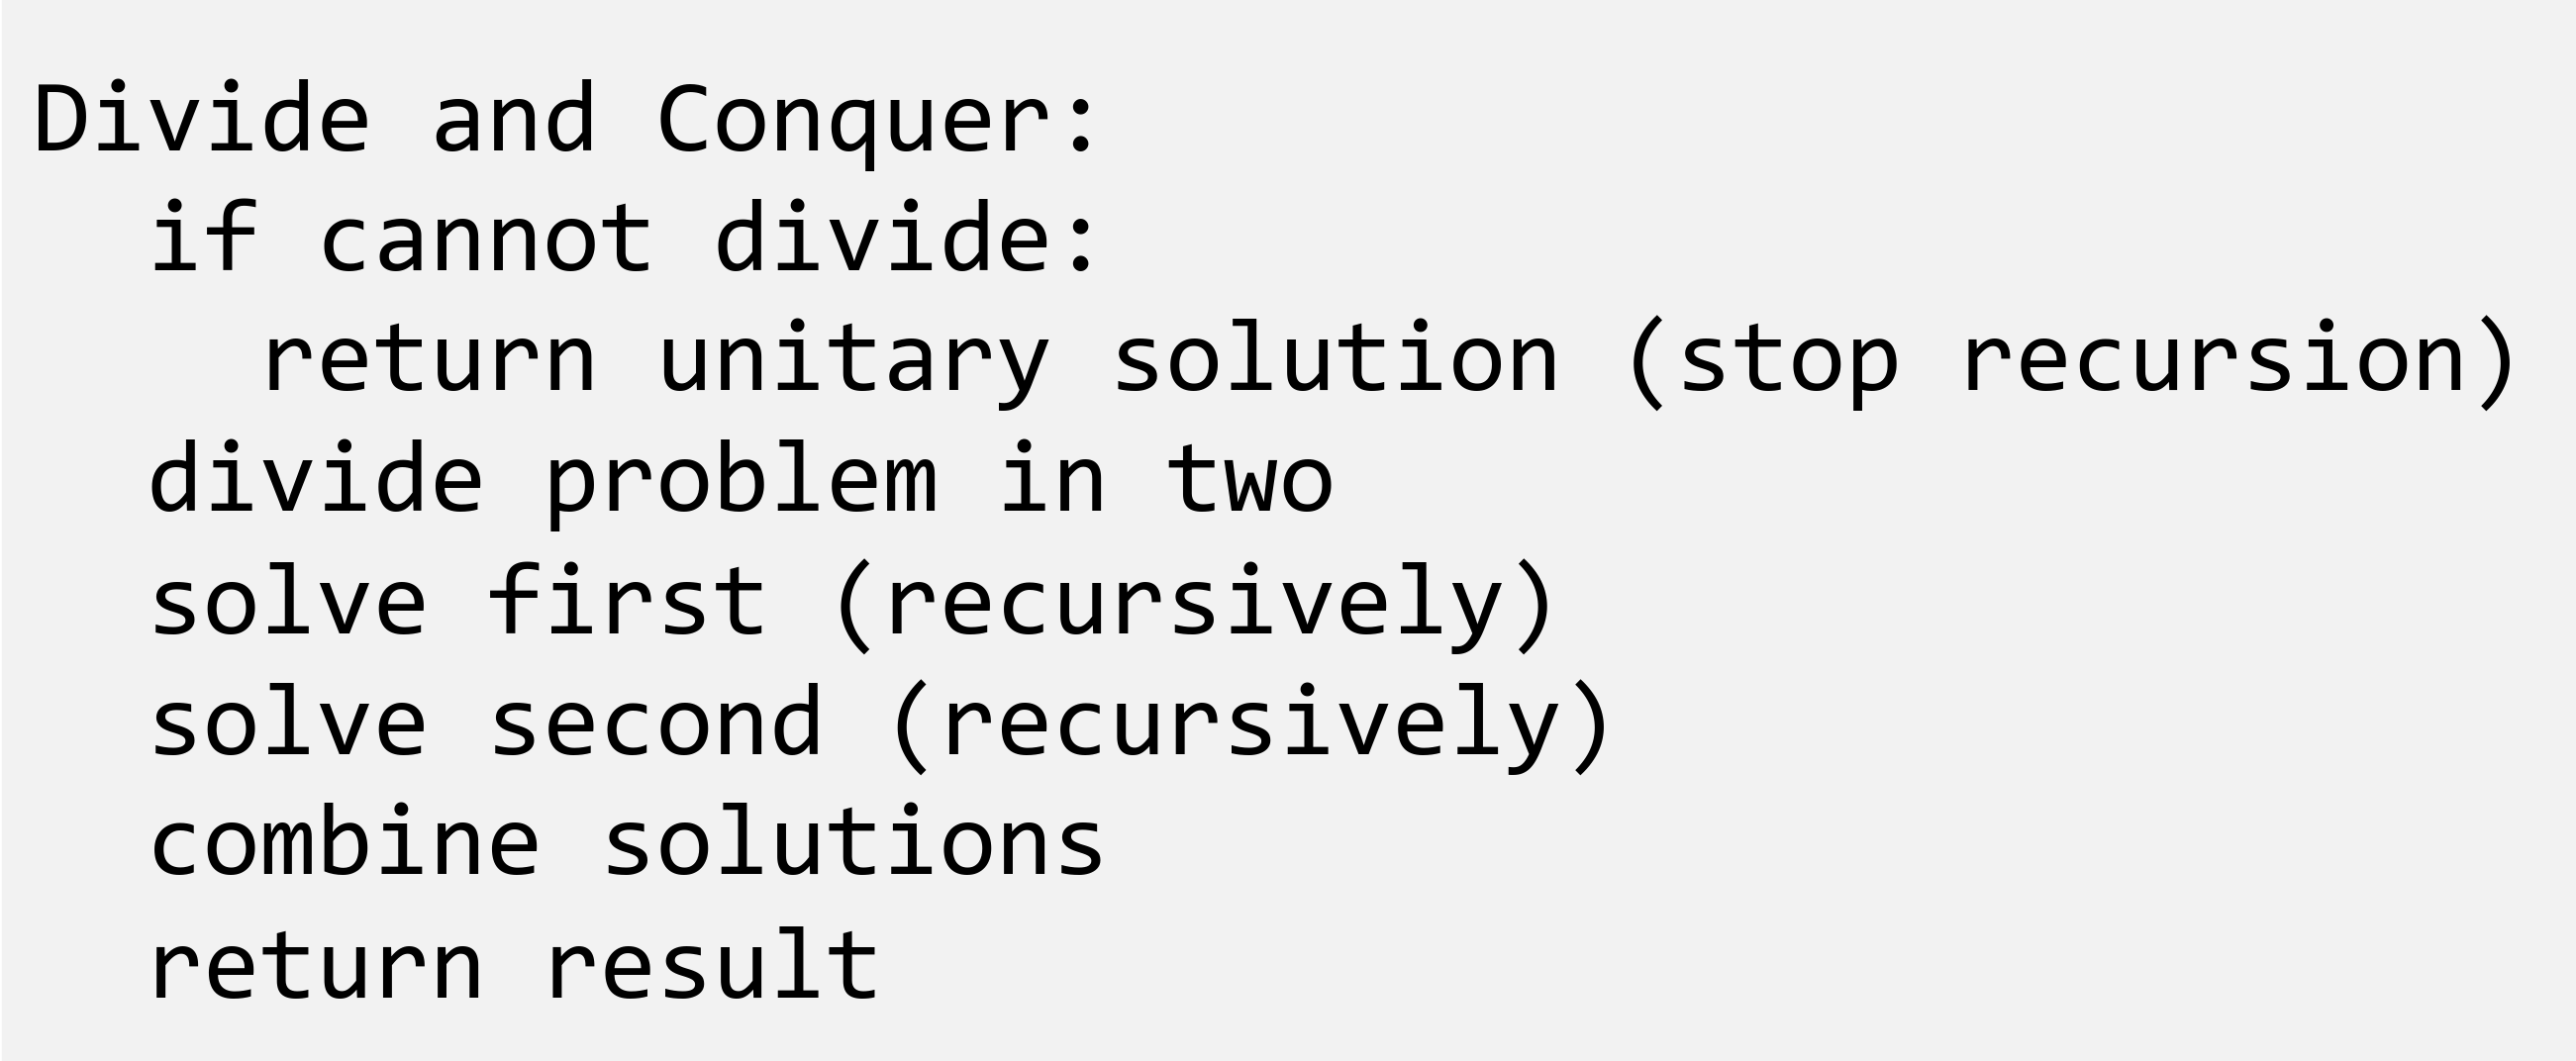
\includegraphics[scale=0.08]{DivideAndConquer.png}
    \caption{Structure of a Divide-and-Conquer Program.}
\end{figure}
\noindent We can implement this with the following code:
\begin{minted}[]{java}
public static int do_sum_rec(int[] arr, int startIdx, int endIdx) {
    int size = endIdx-startIdx;
    if (size == 1) // check for termination criteria
        return arr[startIdx];
    // split array in half and call self recursively
    int mid = size / 2;
    int sum1 = do_sum_rec(arr, startIdx, startIdx + mid);
    int sum2 = do_sum_rec(arr, startIdx + mid, endIdx);
    return sum1 + sum2;
}
\end{minted}
\noindent We can trivially parallelize this by solving the recursion for the first and second subproblem in parallel. We get the following structure of function calls:
\begin{figure}[H]
    \centering
    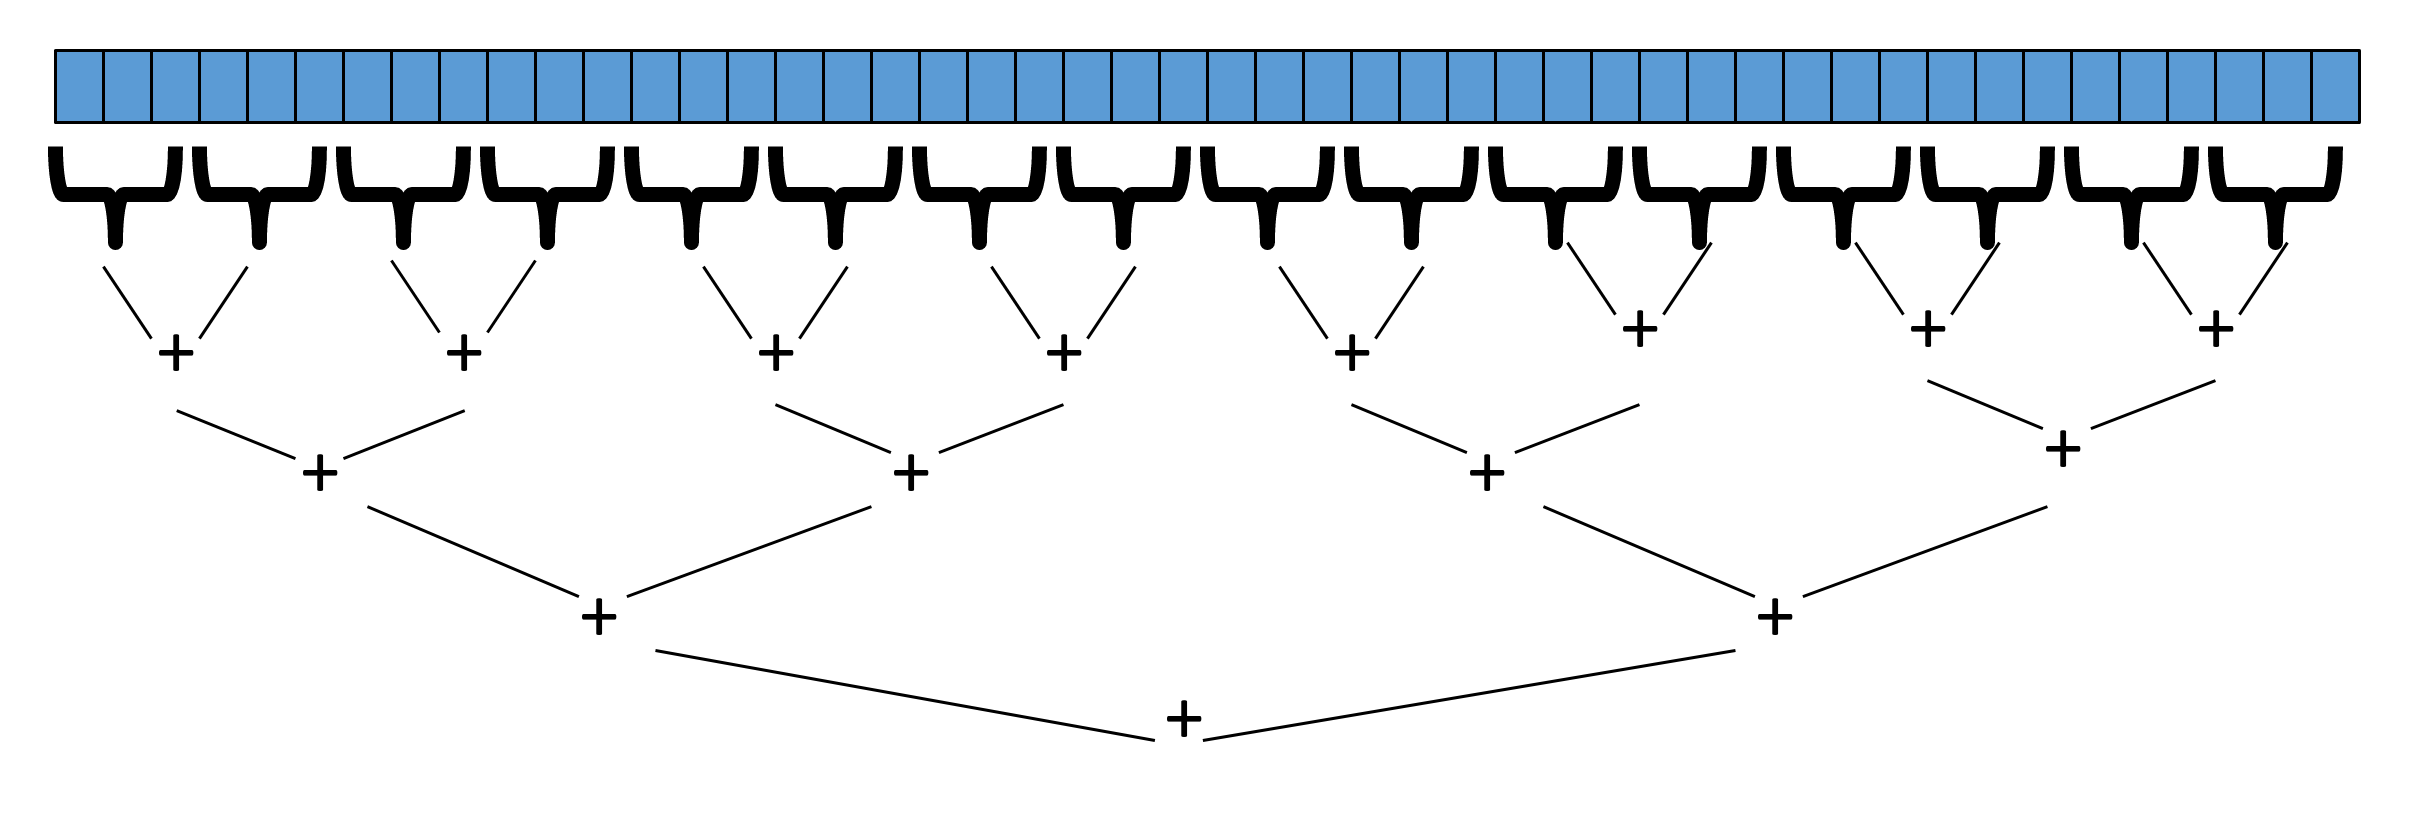
\includegraphics[scale=0.15]{DnCTree.png}
    \caption{Structure of a Divide-and-Conquer Program.}
\end{figure}
\noindent Function calls on the same level in the tree can be executed in parallel. Notice that the tree has a depth logarithmic in the number of array entries. This is much better than what we can achieve by simply dividing up the array between threads.\\
Although to actually get the logarithmic runtime, we require as many processors as array entries. Else, the threads on the last level cannot all run in parallel. This is not realistic, so we cannot expect logarithmic runtime. But this approach is still superior compared to our initial approach with dividing the array into equal chunks, because it solves two previously mentioned problems:
\begin{itemize}
  \item The sequential bottleneck of summing up the partial results is solved since even the result combination is parallelized. We get more speedup, even though a logarithmic runtime is not realistic.
  \item It is easier to implement more equal load balancing. Consider again a graph as an input datastructure. When a task divides up its assigned vertices on two subtasks, it can also count the number of edges in the two sets and adjust the division accordingly (such that both subtasks get not just a similar amount of vertices, but also a similar amount of edges). This is a much simpler problem than when we have to partition the entire graph on \textit{n} threads in the beginning.
\end{itemize}

\newpage

\subsubsection{Parallel Divide-And-Conquer with Java Threads}
But now, how do we implement this parallelization of the two subtasks? Of course we can create two threads solving each half recursively. This would look something like this:
\begin{minted}[]{java}
public void run() {
    int size = endIdx - startIdx;
    if (size == 1) {
        result = arr[startIdx];
        return;
    }
    int mid = size / 2;
    SumThread t1 = new SumThread(arr, startIdx, startIdx + mid);
    SumThread t2 = new SumThread(arr, startIdx + mid, endIdx);
    t1.start();
    t2.start();
    t1.join(); // join() would have to be in a try-catch block
    t2.join();
    result = t1.result + t2.result;
    return;
}
\end{minted}
\noindent Now imagine we want to process arbitrarily large arrays like this. Remember that each Java thread is mapped to an OS thread. Also remember that each OS thread gets some resources, for example a stack. This is a small region of memory residing in main memory. When we now create millions of threads for a large array, we will sooner or later run out of memory. This will be visible with the following error:

\begin{figure}[H]
    \centering
    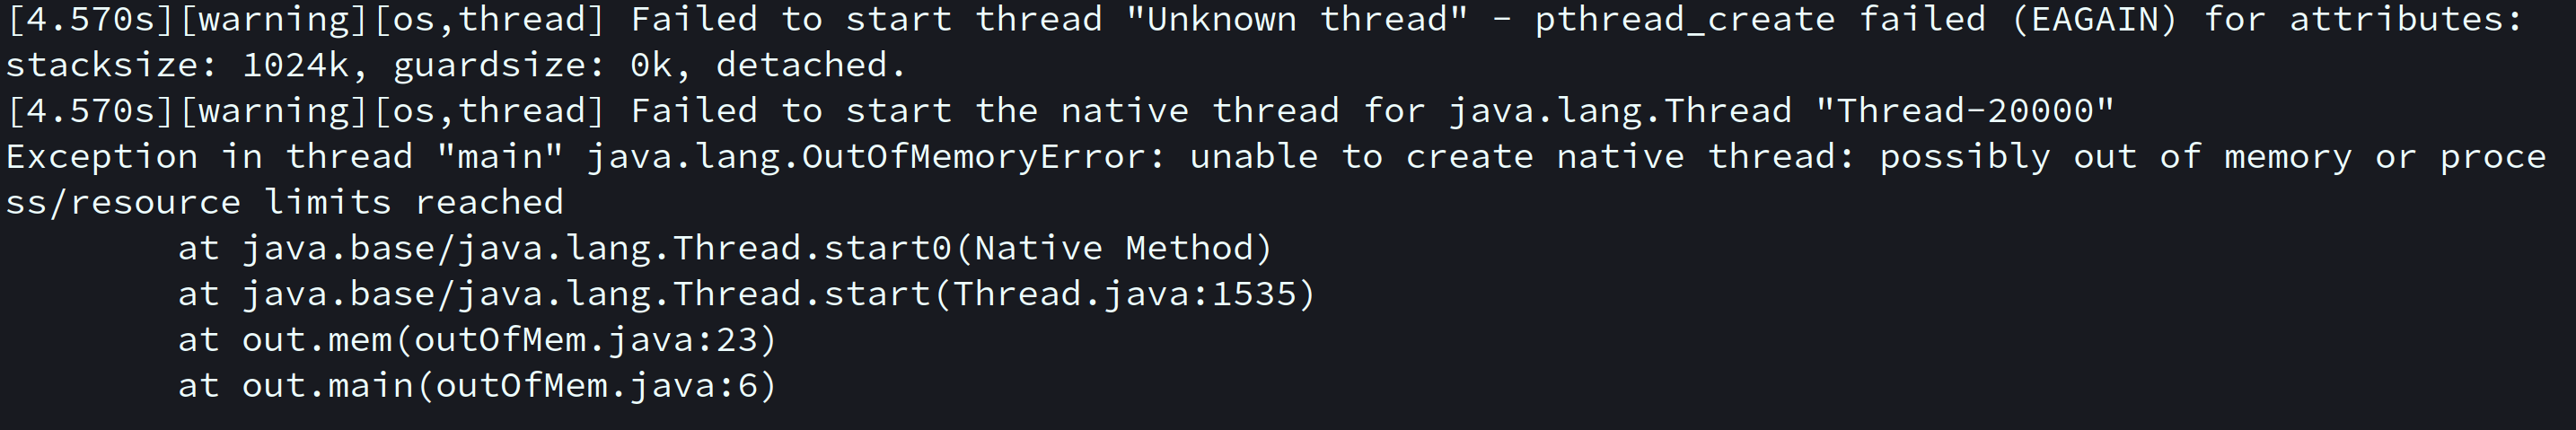
\includegraphics[scale=0.15]{OutOfMem.png}
    \caption{OutOfMemoryError-Exception due to creating too many threads in Java.}
\end{figure}

\noindent Implementing parallel divide-and-conquer with native Java threads is not feasible due to their resource consumption. Using native Java threads for recursive subtasks is not suitable for a number of reasons anyways:

\begin{itemize}
  \item \textbf{Resource blocking:} A thread will join its subthreads and potentially wait for a long time for them to return. In this time, the Java Thread object blocks an OS thread, which may be idle (does not use up CPU time, which is good), but still blocks the resources allocated for the underlying OS thread. When we have millions of threads, most of which are currently joining, large chunks of memory are allocated, even though few threads are doing actual work.
  \item \textbf{Many more threads than cores:} We probably do not have millions of cores to run the code on. Therefore, we cannot possibly gain an advantage by creating so many (Java and thus OS) threads. Remember that creating OS threads brings some overhead. Also, context switching between the threads is expensive, so we never want to have many more active OS threads than we have processors.
\end{itemize}

\noindent The problem we have is fundamentally that Java threads are too \textit{heavy-weight} for these recursive tasks. The recursive tasks do not each require their own OS thread, which is what is given to them when we create Java threads. Remember that in chapter 1, we said that many languages have something like virtual threads. That is, the user creates virtual threads (or tasks) and the language runtime decides itself how these are going to be mapped to OS threads. The advantage is that by using this approach, the virtual threads are (potentially) much less heavy-weight than when simply one-to-one mapping to OS threads, solving all of our problems.

\subsubsection{Manually Optimizing Divide-And-Conquer using Java Threads}
Before we look into solutions to this problem of Java threads being too heavy-weight, let us perform two manual optimizations:

\begin{enumerate}
  \item Currently, we break down the problem until the assigned chunk size equals one. This is not efficient, as thread creation brings some overhead. Say we process a chunk of 20 array elements. When we divide this onto two new threads, each only has to process 10 elements. However, the time required to create and start new threads is significantly longer than the time gained to process 10 instead of 20 elements. Hence, we introduce a \textbf{cutoff} at, say, 1000 elements. As soon as the assigned array chunk has length less than 1000, the thread will sum it itself and not divide it any further. Using this optimization, we need to create fewer threads.
  \item When we create two threads to solve each half of the problem, the thread creating them has nothing to do while waiting on the two results but still blocks resources. It would be more efficient when the thread solves one half itself and outsources the second half to another thread to solve concurrently. We can do this by calling \texttt{Thread.run()} instead of \texttt{Thread.start()}. This again means that we need to create fewer threads.
\end{enumerate}

\noindent Using these two optimizations, we receive the following code:

\begin{minted}[]{java}
public void run() {
    int size = endIdx - startIdx;
    if (size <= 1000) {
        result = 0;
        for (int i = startIdx; i < endIdx; i++) {
            result += arr[i];
        }
        return;
    }
    int mid = size / 2;
    SumThread t1 = new SumThread(arr, startIdx, startIdx + mid);
    SumThread t2 = new SumThread(arr, startIdx + mid, endIdx);
    t1.start();
    t2.run(); // executes the run() method of t2 with the current thread
    t1.join(); // join() would have to be in a try-catch block
    result = t1.result + t2.result;
    return;
}
\end{minted}

\noindent Even with these optimizations, our problem with Java threads being too heavy-weight remains due to resource-blocking, creation and context switching overhead. These optimizations simply mean that we create less threads overall, but for sufficiently large arrays, the exact same problems occur.

\subsubsection{Solving Heavy-Weight Threads in Java: ExecutorService}
\label{ExecutorService}
Java provides us the \texttt{ExecutorService} framework as an abstraction layer between tasks and threads. Instead of creating a thread to solve one half of the array recursively, we create a \textit{task} and submit it to an \texttt{ExecutorService}. The \texttt{ExecutorService} then maps these tasks to Java threads itself. This scheduling of tasks to Java threads is similar to what the OS does on a lower abstraction level, where it maps OS threads to available processors.\\[3mm]
This seems to be exactly what we need to solve our issue with the heavy-weight Java threads. Let us create an \texttt{ExecutorService} instance in Java:
\begin{minted}[]{java}
// Create an ExecutorService with a fixed thread pool of 4 threads
ExecutorService executor = Executors.newFixedThreadPool(4);
\end{minted}
\noindent Here, we give the \texttt{ExecutorService} instance a pool of four threads. This means that the service will create four threads when initialized. When we now submit tasks, these will wait in a queue for a thread in the pool to become available.
\begin{figure}[H]
    \centering
    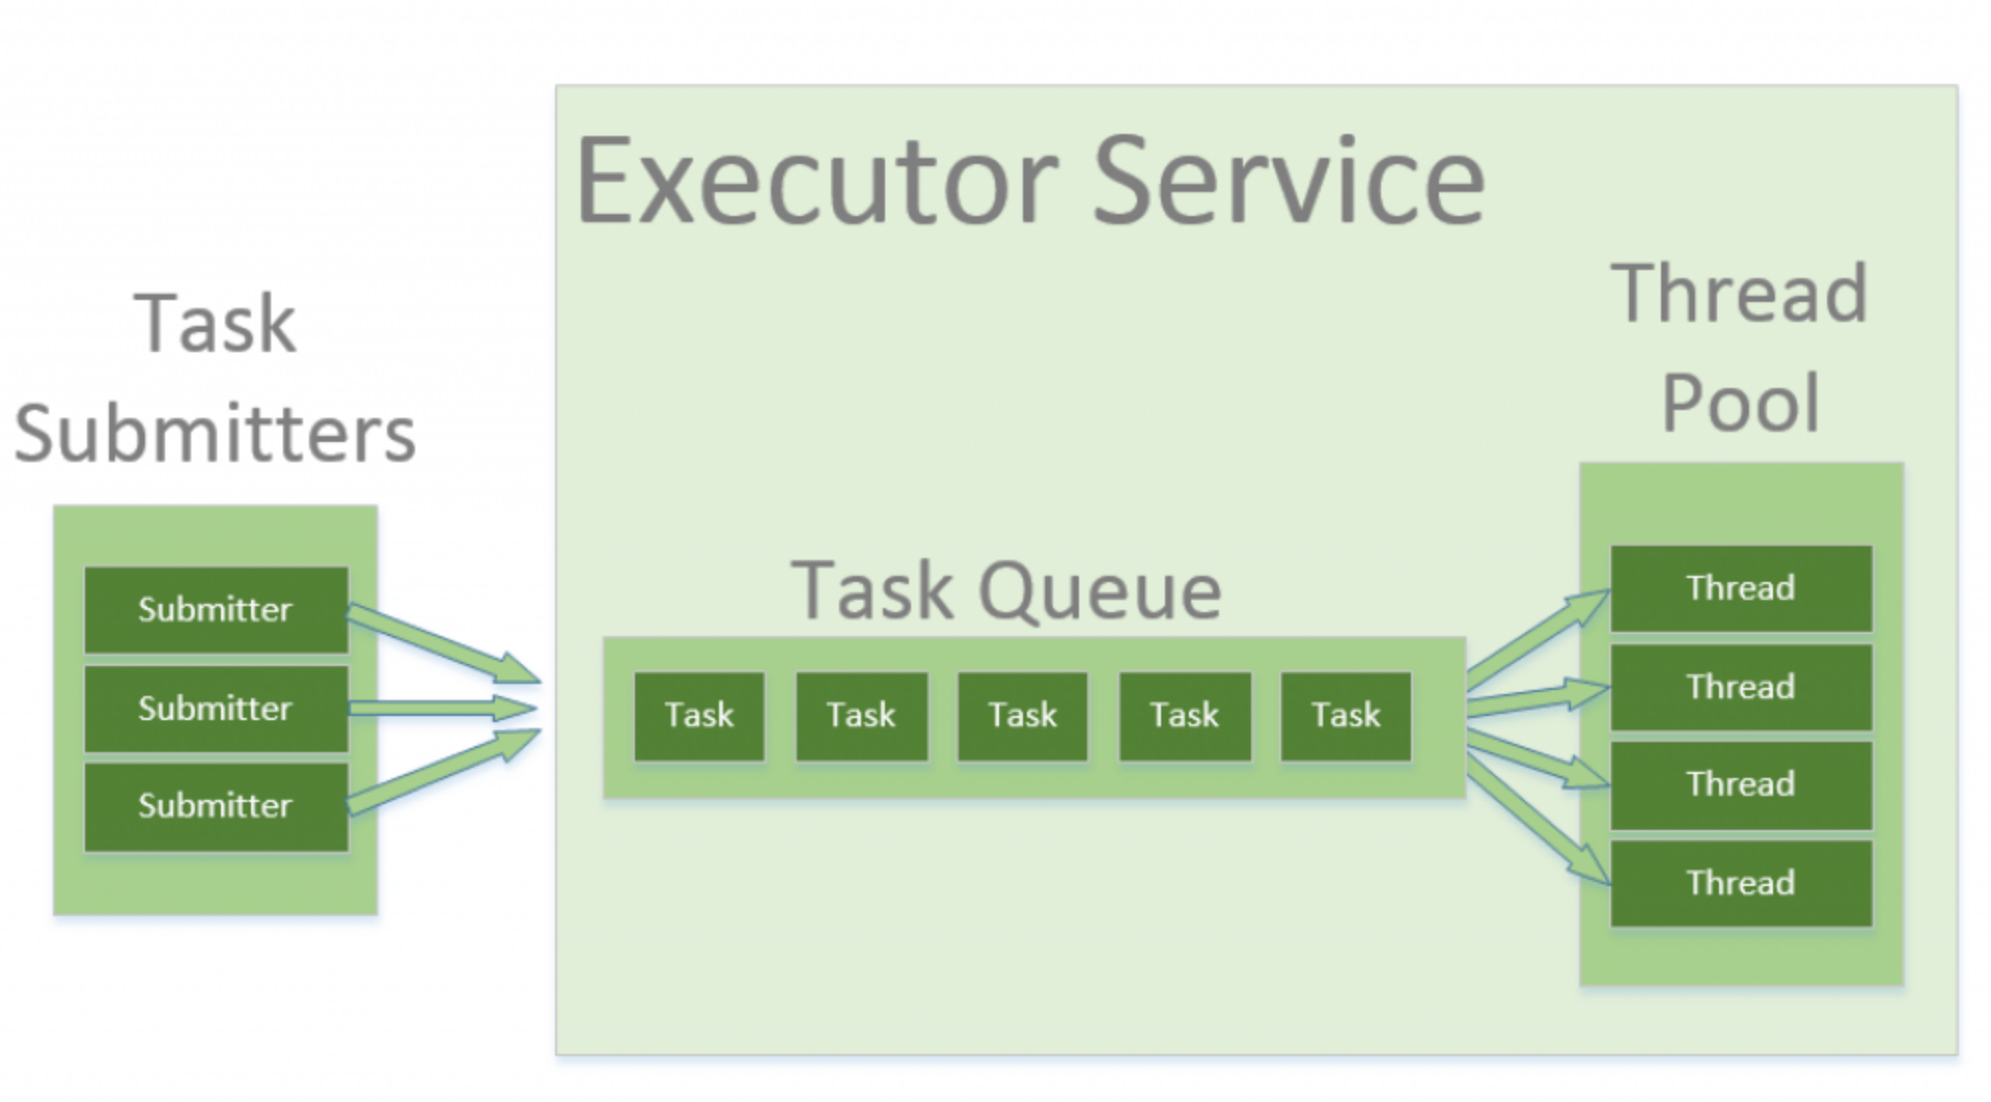
\includegraphics[scale=0.13]{ExecutorServiceQueue.png}
    \caption{Internal structure of \texttt{ExecutorService} with a fixed thread pool: https://www.baeldung.com/thread-pool-java-and-guava}
\end{figure}
\noindent What exactly do we submit to the \texttt{ExecutorService} now? Threads? Almost. Remember that we could create a Java Thread object by initializing it with a \texttt{Runnable} object? We can submit exactly such \texttt{Runnable} objects to the \texttt{ExecutorService} (and also others). Some important methods of \texttt{ExecutorService} are the following. Let \textit{ex} be an \texttt{ExecutorService} instance in our code.
\begin{itemize}
  \item \texttt{ex.submit(Runnable task)}: Submits a Runnable object for execution and returns a Future object representing that task.
  \item \texttt{ex.submit(Callable<T> task)}: Submits a value-returning task for execution and returns a Future object representing the pending results of the task. This allows us to submit a \texttt{Callable<T>} object (think of a Runnable object that can return a value of type T and implements the \texttt{call()} function instead of the \texttt{run()} function).
  \item \texttt{ex.shutdown()}: Initiates an orderly shutdown in which previously submitted tasks are executed, but no new tasks will be accepted. After all previously submitted tasks are executed, the thread pool is deallocated. We always call this method when we finish using the \texttt{ExecutorService} instance.
\end{itemize}
\noindent When we submit tasks, \texttt{ExecutorService} returns us a Future object. This provides us a handle for the submitted task to for example request the result or check its progress. Let us write a simple program using \texttt{ExecutorService} to get a better idea of what we can do.

\begin{minted}[]{java}
public static void main(String[] args) {
    /* submit 100 callables to the service and store the returned
     Future objects in a list */
    ExecutorService ex = Executors.newFixedThreadPool(4);
    List<Future<Integer>> futures = new ArrayList<>();
    for (int i = 0; i < 100; i++) {
        Future<Integer> future = ex.submit(new MyCallable());
        futures.add(future);
    }

    // sum up the results of all tasks
    int sum = 0;
    for (Future<Integer> future : futures) {
        try {
            sum += future.get();
        } catch (InterruptedException | ExecutionException e) {
            e.printStackTrace();
        }
    }

    System.out.println("Sum of all results: " + sum);
    ex.shutdown();
}
\end{minted}

\newpage

\begin{minted}[]{java}
class MyCallable implements Callable<Integer> {
    /* implement the call() method. The call() method is the code the task
     executes when it is its turn */
    public Integer call() throws Exception {
        int sum = 0;
        for (int i = 0; i < 10; i++) {
            sum += i;
        }
        return sum;
    }
}
\end{minted}

\noindent We can see that when calling \texttt{future.get()}, we get the result of the computation. When using threads, we first need to call \texttt{thread.join()} to ensure the computation is completed. But here, the underlying threads are abstracted away and calling \texttt{future.get()} automatically waits on the task being finished, without having to join.

\subsubsubsection{Parallel Divide-And-Conquer with \texttt{ExecutorService}}
With \texttt{ExecutorService}, we can now try implementing our parallel divide-and-conquer program again. Since we can create a fixed thread pool, we will not have the same issue of running out of memory, no matter the array size. Let us implement the \texttt{call()} method of a corresponding \texttt{Callable} class using \texttt{ExecutorService}:
\begin{minted}[]{java}
public class SumRecCall implements Callable {
    ...

    public Integer call() throws Exception {
        int size = endIdx - startIdx;
        if (size <= 1000) {
            int result = 0;
            for (int i = startIdx; i < endIdx; i++) {
                result += arr[i];
            }
            return result;
        }
        int mid = size / 2;
        SumRecCall c1 = new SumRecCall(ex, arr, startIdx, startIdx + mid);
        SumRecCall c2 = new SumRecCall(ex, arr, startIdx + mid, endIdx);
        Future<Integer> f1 = ex.submit(c1);
        Future<Integer> f2 = ex.submit(c2);
        return f1.get() + f2.get();
    }

    ...

}
\end{minted}

\begin{minted}[]{java}
// main method defined somewhere else
public static void main(String[] args) {
    ExecutorService ex = Executors.newFixedThreadPool(4);
    SumRecCall task = new SumRecCall(ex, arr, 0, arr.length);
    Future<Integer> result = ex.submit(task);
    System.out.println(result.get());
    ex.shutdown();
}
\end{minted}
\noindent When we now run this program, we notice that it does not return. To understand what happens, let us consider the workings of \texttt{ExecutorService} again. A submitted task is put in a wait queue, where it waits until one of the four threads in the pool is free. Now, let us consider what happens with the first five tasks submitted in this code:
\begin{itemize}
  \item The first task gets the whole array to process, hence it creates and submits two further tasks to process each half. However, this first task is assigned to the first thread in the pool. It will keep occupying this thread, even when it now has to wait for its subtasks to complete.
  \item The two tasks created by the first task occupy the second and third thread in the pool, meaning only one thread remains free. Since the array is presumably quite long, these two tasks will again create two more tasks each (to solve each of their problem half) and submit them to the service. Again, even though they are waiting for a Future to return its result, they all occupy a thread in the pool and will not let it go until they completed their \texttt{call()} method.
  \item Task four will get the last thread in the pool. The fifth task that is submitted will not find a free thread in the pool anymore. That means that it will wait in the queue for a thread to become free. However, this will not happen, as the tasks currently occupying the thread are waiting for the tasks in the queue to return their result. They of course cannot do this without a thread. We have reached a deadlock.
\end{itemize}
This seems very disappointing at first. The fixed thread pool of the executor service is not made for tasks that create further tasks themselves. An example for a useful application using \texttt{ExecutorService} is handling HTTP requests of a webserver. Each request is submitted to the \texttt{ExecutorService} as a task and the service distributes the tasks across the available threads.

\subsubsection{Java Fork/Join Framework}
When we browse the Java documentation, we find that \texttt{ExecutorService} is an interface. Remember that interfaces in Java define some high-level behaviour by declaring methods that classes can then specifically implement. We can instantiate an \texttt{ExecutorService} for example through the fixed thread pool we saw earlier. There is another interesting implementation of the \texttt{ExecutorService} interface called \texttt{ForkJoinPool}. This class is the center of Java's Fork/Join framework and designed for recursive tasks, exactly what we are looking for. We can instantiate a \texttt{ForkJoinPool} in the following way:

\begin{minted}[]{java}
ForkJoinPool fj = new ForkJoinPool(4);
fj.invoke(new Task());
fj.shutdown();
\end{minted}

\noindent Assuming that the class \texttt{Task} is some kind of generic task the \texttt{ForkJoinPool} accepts, this code creates a \texttt{ForkJoinPool} that uses a maximum of four Java threads and starts a \texttt{Task} object. With our previous knowledge, we can characterize the \texttt{ForkJoinPool} class with a few points:

\begin{itemize}
  \item A \texttt{ForkJoinPool} is an implementation of the \texttt{ExecutorService} interface. We can instantiate it (among other possibilities) by specifying the maximum number of used Java threads as an argument.
  \item The difference to the \texttt{ExecutorService} thread pools we previously saw is that it employs \textbf{work stealing}. We will elaborate on this, but in a nutshell, it means that instead of simply waiting for subtasks to finish, threads in the Fork/Join Framework steal tasks from other threads to execute in the meantime. This is the key feature that prevents the deadlock problem we previously had with \texttt{ExecutorService}.
  \item The tasks that a \texttt{ForkJoinPool} accepts are \texttt{ForkJoinTask}s. The \texttt{ForkJoinTask} class is an abstract base class, with the relevant subclasses being \texttt{RecursiveTask<V>} and \texttt{RecursiveAction} (similar to \texttt{Callable<T>} and \texttt{Runnable}). So, we invoke our \texttt{ForkJoinPool} usually with either a \texttt{RecursiveTask<V>} (when we require our tasks to return a value of type V) or a \texttt{RecursiveAction} object (if no return value is required).
  \item To start subtasks from within a task, we can call \texttt{ForkJoinTask.fork()} and then \texttt{ForkJoinTask.join()} to wait for the computation to be finished.
\end{itemize}

\subsubsubsection{Parallel Divide-And-Conquer with Fork/Join Framework}
\noindent Let us now finally implement our parallel array sum algorithm using the Fork/Join framework:

\begin{minted}[]{java}
public int sumArray(int[] arr) {
    ForkJoinPool fj = new ForkJoinPool(4);
    SumRecCall sumTask = new SumRecCall(arr, 0, arr.length);
    int result = fj.invoke(sumTask);
    fj.shutdown();
    return result;
}
\end{minted}

\begin{minted}[]{java}
class SumRecCall extends RecursiveTask<Integer> {
    int[] arr;
    int endIdx, startIdx;

    // constructor
    public SumRecCall(int[] arr, int startIdx, int endIdx) {
        this.arr = arr;
        this.startIdx = startIdx;
        this.endIdx = endIdx;
    }

    public Integer compute() {
        int size = endIdx - startIdx;
        if (size <= 1000) {
            int result = 0;
            for (int i = startIdx; i < endIdx; i++) {
                result += arr[i];
            }
            return result;
        }
        int mid = size / 2;
        SumRecCall first = new SumRecCall(arr, startIdx, startIdx + mid);
        SumRecCall second = new SumRecCall(arr, startIdx + mid, endIdx);
        first.fork();
        second.fork();
        int firstSum = first.join();
        int secondSum = second.join();
        return firstSum + secondSum;
    }
}
\end{minted}

\noindent We see that the syntax is similar to our previous approach using a fixed thread pool for an \texttt{ExecutorService}. Differently though, we do not need to store a \texttt{Future} object returned by the task. This is because the \texttt{RecursiveTask} \textit{is} the \texttt{Future} object (the \texttt{RecursiveTask} and \texttt{RecursiveAction} classes implement the \texttt{Future} interface). Hence, we can simply get the result by calling \texttt{ForkJoinTask.join()}.\\[3mm]
Note that we could compute one half on the current thread by calling \texttt{second.compute()} instead of \texttt{second.fork()} to perform the same manual optimization as we did when using Java threads. However, this provides us no advantage in the Fork/Join framework as the task scheduler of the framework optimizes this by itself. So, we can neatly \texttt{fork()} and \texttt{join()} both tasks and need not worry about performance.\\
However, the optimization to set a sequential cutoff is still important to make sure each task provides enough work. This is because while we do not create a new thread for each task anymore, there is still some overhead to enqueue this task and schedule it on the worker threads in the pool. Setting the threshold to something like 1000 array elements is reasonable in this case to strike a good balance between exploiting parallelism and ensuring the task creation overhead does not dominate execution time.

\subsubsubsection{Work-Stealing in the Fork/Join Framework}
We mentioned that the Fork/Join framework solves the deadlock problem other \texttt{ExecutorService} implementations have by means of employing a work-stealing algorithm for scheduling submitted tasks among threads in the pool.\\[3mm]
Remember from \ref{ExecutorService} (\texttt{ExecutorService} introduction) that the submitted tasks within an \texttt{ExecutorService} enter a queue where they wait for a free thread in the pool. The Fork/Join framework now implements work-stealing in the following way:

\begin{itemize}
  \item Each thread in the \texttt{ForkJoinPool} additionally maintains its own queue of assigned tasks.
  \item When a thread in the pool runs out of tasks (i.e. its queue becomes empty), it attempts to \textit{steal} tasks from the queues of other threads in the pool.
  \item When a thread in the pool encounters a \texttt{ForkJoinTask.join()} operation (meaning it has to wait for the result/termination of the computation) it processes other tasks from the queue until the joined task is finished.
\end{itemize}

\noindent With this additonal queue per thread and the threads processing other tasks upon a \texttt{join()} operation, the recursion required by parallel divide-and-conquer is finally possible in an efficient manner.

\subsubsection{Cilk}
Cilk is a programming language developed at MIT in the 1990s. Based on the C programming language, the idea behind Cilk was to extend C to better support multi-threaded programming. You might ask now why we even talk about Cilk in this course, as we already use Java. We are not concerned with actually learning the Cilk language or understanding its exact implementation details.\\
Cilk is relevant for us as it pioneered a specific programming style of spawning and joining tasks (i), using a work-stealing scheduler to map these tasks to available processors (ii), providing strong runtime guarantees based on this scheduling (iii) and introducing a multi-threaded computation model (iv). If you noticed that this sounds a lot like the Java Fork/Join framework, you are right. The Fork/Join framework in Java is based heavily on the Cilk language and thus we can learn a lot about it by studying the ideas behind Cilk.\\
The basis of Cilk-style programming is that the programmer expresses parallelism by spawning tasks and then joining them (waiting for results). A core of the project was to support Fork/Join parallelism by implementing a suitable task scheduler. The idea being that the programmer is concerned with the structure of the program (which tasks to spawn and join) and the scheduler is concerned with efficiently mapping these spawned tasks to available processors.


\subsubsubsection{The Cilk Model of Multi-Threaded Computation}
Closely tied to the Cilk programming style with spawning and joining tasks, Cilk also introduced a graph computation model that allows us to reason about runtime bounds. To introduce the model, we consider the following pseudo-code of the exponential Fibonacci algorithm:

\begin{minted}[]{java}
public long fib(int n) {
    if (n < 2)
        return n;
    spawn task for fib(n-1);
    spawn task for fib(n-2);
    wait for tasks to complete
    return addition of results
}
\end{minted}

\noindent In the Java Fork/Join framework, the two spawns would correspond to \texttt{ForkJoinTask.fork()} operations and the wait to \texttt{ForkJoinTask.join()} operations.\\
We now consider the computation of \texttt{fib(4)}. We can model the program execution as a dag (directed acyclig graph) by:

\begin{itemize}
  \item Creating vertices for each \texttt{spawn} and \texttt{wait}.
  \item Grouping vertices within the same function call (for example within a call to \texttt{fib(3)}) into a \textbf{procedure} block.
  \item Creating a \textbf{spawn edge} for each spawn call, a \textbf{return edge} for each wait and a \textbf{continuation edge} for a step within the same function call (procedure).
\end{itemize}

\newpage

\noindent We receive the following execution graph:

\begin{figure}[H]
    \centering
    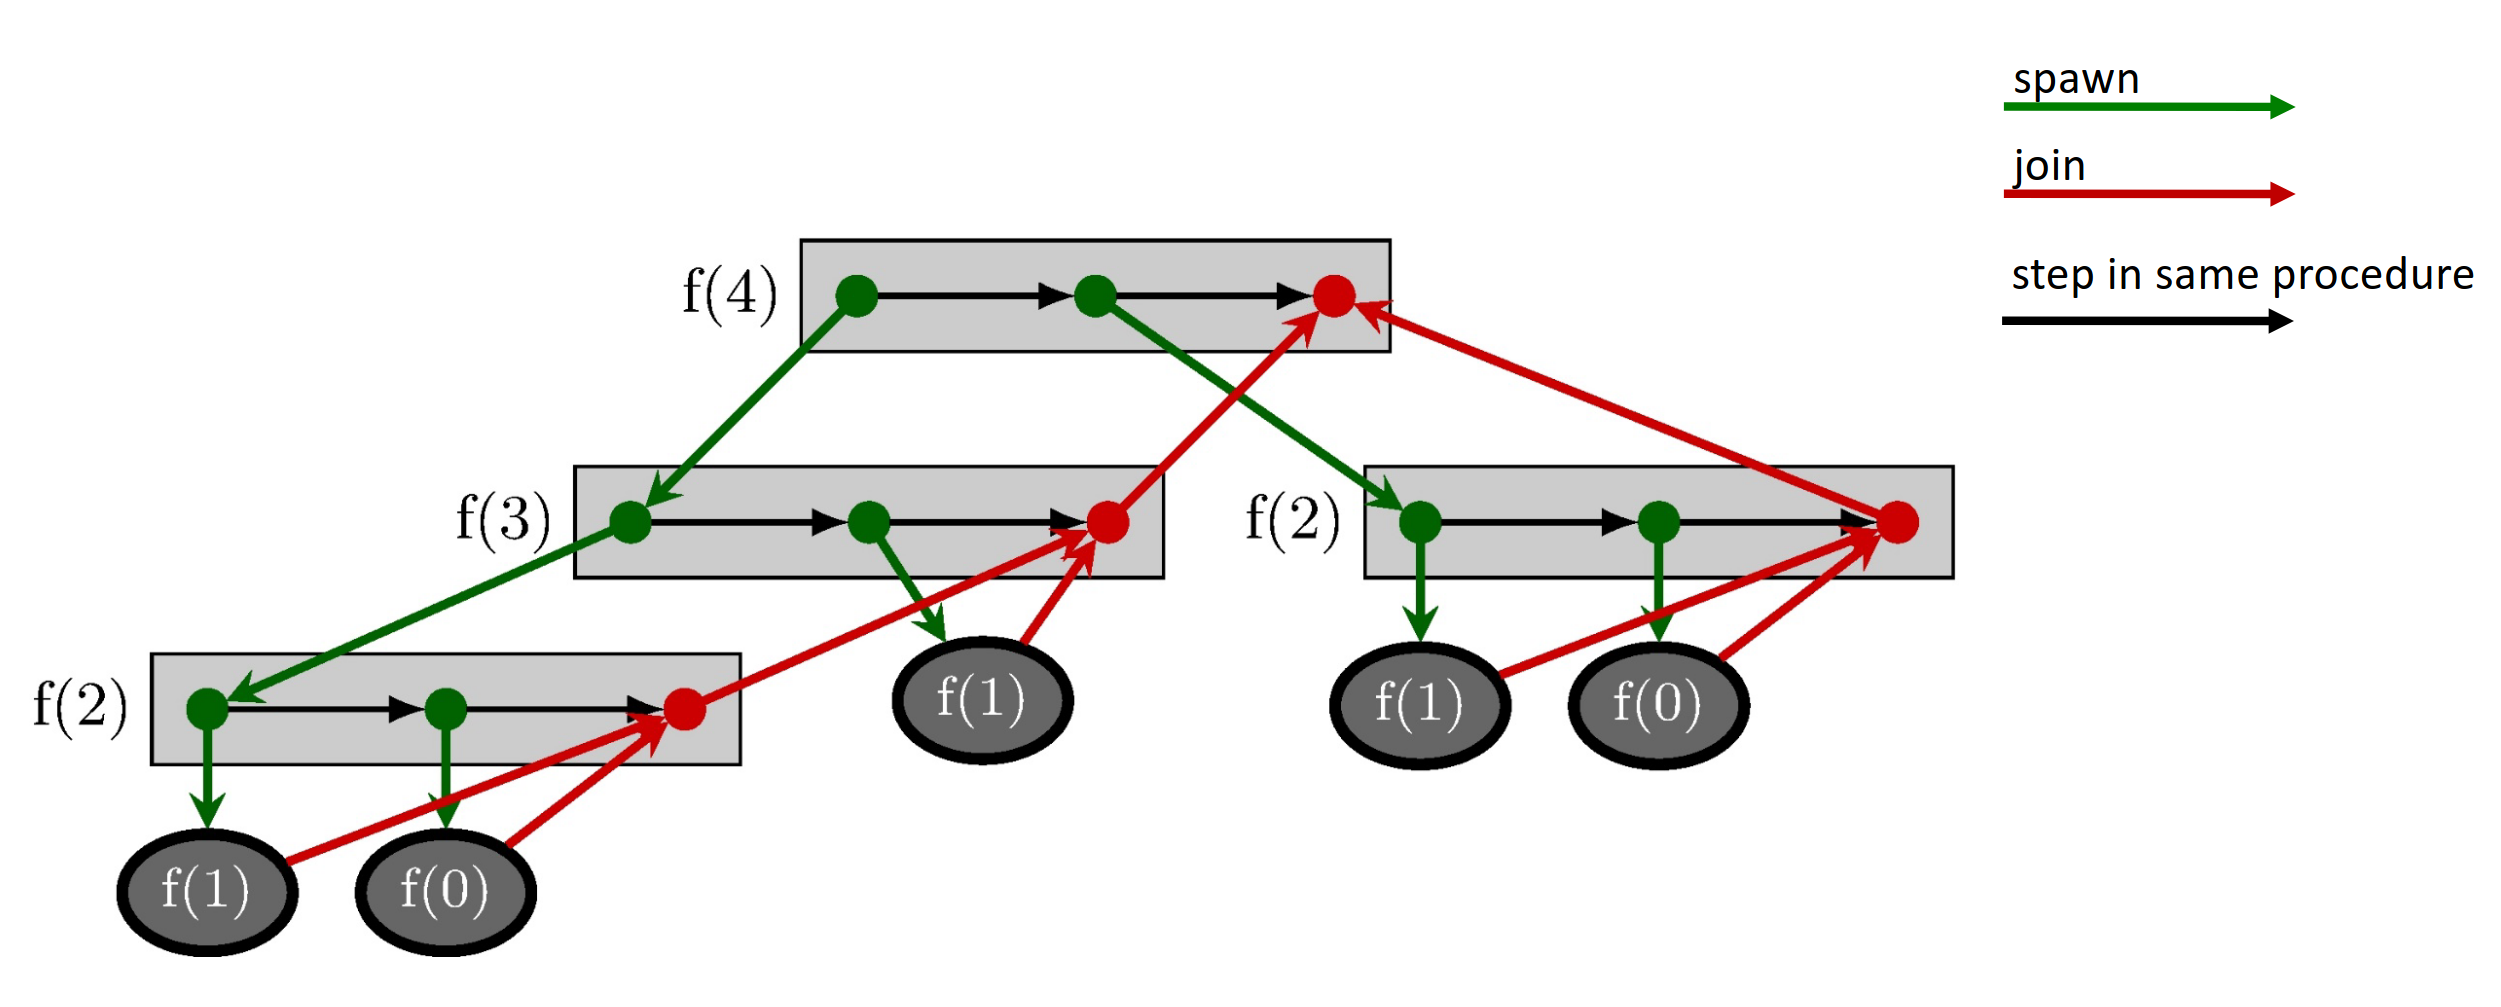
\includegraphics[scale=0.15]{FibTaskGraph.png}
    \caption{Cilk Graph of Fib(4) execution.}
\end{figure}

\noindent In each procedure (\texttt{Fib(n)} call), we have three vertices corresponding to two spawns and one wait. Exceptions are the leaves, which correspond to the base cases (\(n < 2\)) and thus immediately return without any vertices.

\subsubsubsection{Task Graphs}
The Cilk model of multi-threaded computation is an example of a task graph model. Such models help us visualize and understand dependencies in the code to see where we can exploit parallelism. We can simplify the Cilk model to model each procedure as a vertex and only model the spawn edges. The \texttt{Fib(4)} execution would then look like this:

\begin{figure}[H]
    \centering
    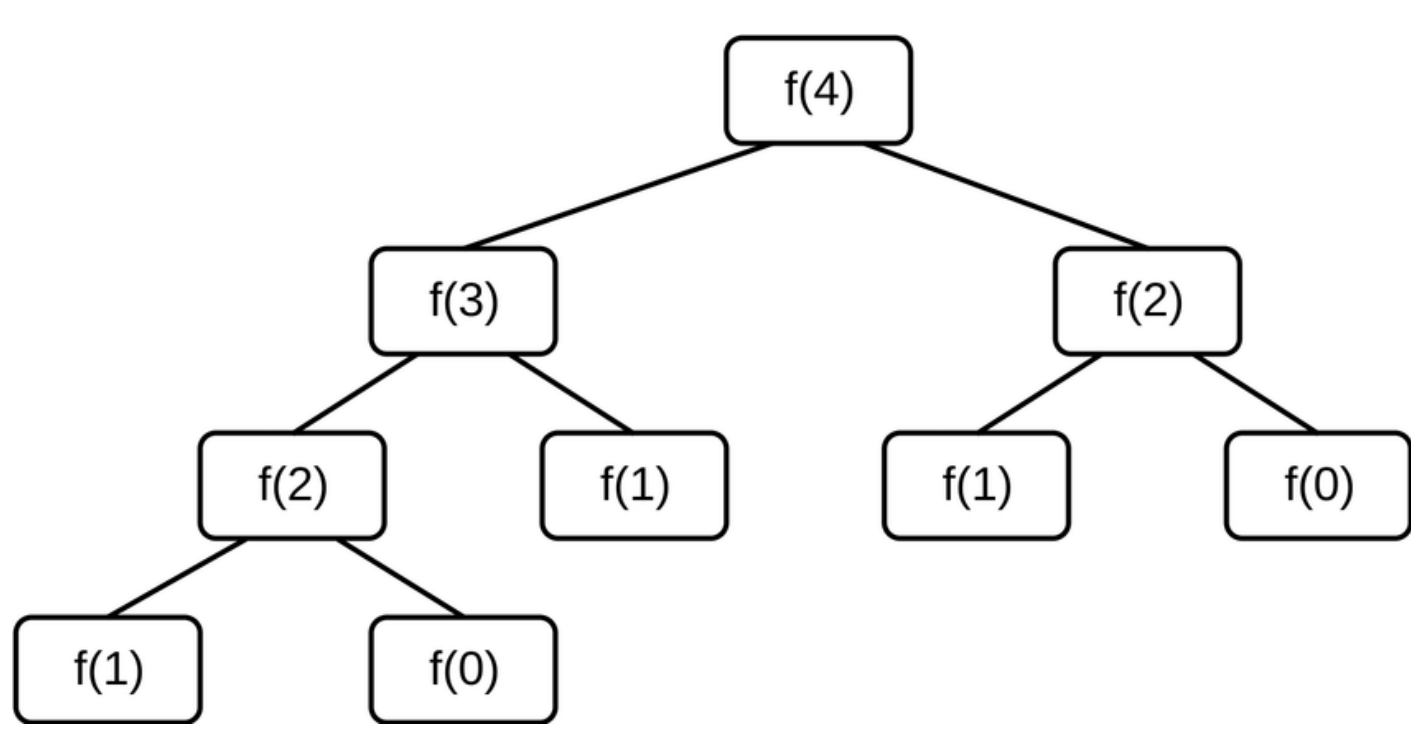
\includegraphics[scale=0.17]{FibSimpleTaskGraph.png}
    \caption{Simple Task Graph of Fib(4) execution.}
\end{figure}

\noindent With such a simple model, we sacrifice some precision in the dependencies, but we can reason about performance bounds in a more straight-forward manner.\\
Let us define that each vertex (task) takes one unit of time to execute. Then, \(T_{1} = n\), where n is the number of vertices in the task graph. This is because a single processor needs to sequentially execute one vertex after the other.\\
We can see that this kind of task graph is a dag. Branches of this dag have no dependencies between each other and could thus be executed in parallel. This also means that intuitively, the \textit{wider} the task graph, the more parallelism can be exploited.\\[3mm]
We notice that no matter how many processors we have, we are limited by the longest path in the graph. This is because each vertex in the path depends on its predecessor. Thus, each path (and in particular the longest path) has to be executed sequentially. Based on this observation, we can define the following:

\begin{definition}
  The \textbf{Critical Path} of a task graph is its longest path. The \textbf{Span} \(=T_{\infty}\) is the length of the critical path, that is, the time required to execute all vertices along the critical path.
\end{definition}

\noindent In our simple model where each vertex takes exactly one unit of time to execute, the span is thus simply the number of vertices lying on the longest path. In the case of our \texttt{Fib(4)} task graph, the span is four. With the span, we can define \textit{parallelism} within a task graph or program:

\begin{definition}
  \textbf{Parallelism} is the maximum possible speedup \(\frac{T_{1}}{T_{\infty}}\).
\end{definition}

\noindent This definition of parallelism formalizes our intuition that a wider task graph equates better parallelism, since a wider graph means more total vertices (i.e. \(T_{1}\) increases), but generally not more depth (i.e. \(T_{\infty}\) stays constant).\\[3mm]
With the definition of span we can also formulate the \textit{span law}:

\begin{theorem}
  \textbf{Span law}: \(T_{P}\geq T_{\infty}\)\\
  That is, any execution using P processors is lower bounded by the span of the task graph.
\end{theorem}

\noindent The law follows trivially from the fact that the span is equal to the execution time on an infinite number of processors \(T_{\infty}\) and thus any execution on any finite number of processors P cannot be faster than this.\\[3mm]
We can also formulate the \textit{work law}:

\begin{theorem}
  \textbf{Work law}: \(T_{P}\geq \frac{T_{1}}{P}\)\\
  That is, P processors require at least \(\frac{T_{1}}{P}\) time to execute all vertices in the task graph.
\end{theorem}

\noindent This is because in each unit of time, each processors can execute at most one vertex (due to dependencies, it might be less than one per processors).\\
We can only give bounds on \(T_{p}\) because it depends on how we schedule the vertices (tasks) on the available number of processors. Let us illustrate this on the following task graph:

\begin{figure}[H]
    \centering
    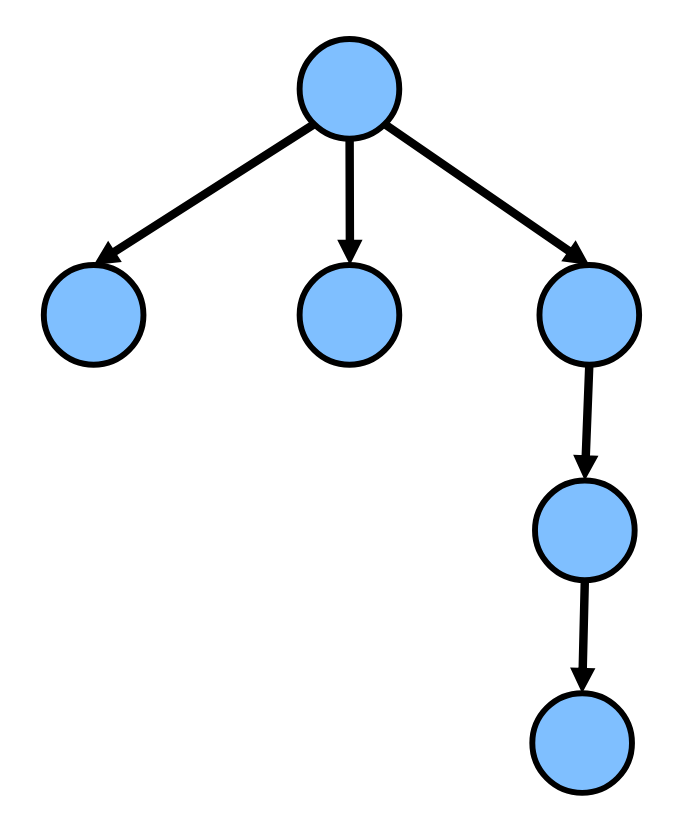
\includegraphics[scale=0.17]{ScheduleTaskGraph.png}
\end{figure}

\noindent What is \(T_{2}\) here? Using our previously deduced bounds, the \textit{work law} tells us that \(T_{2}\geq \frac{6}{2}=3\) since \(T_{1}=6\) and the \textit{span law} tells us that \(T_{2}\geq 4\), since the critical path has length four. However, the exact value of \(T_{2}\) depends on the scheduling we choose. Consider the following two possible schedulings:

\begin{figure}[H]
    \begin{subfigure}[t]{.5\textwidth}
        \centering
        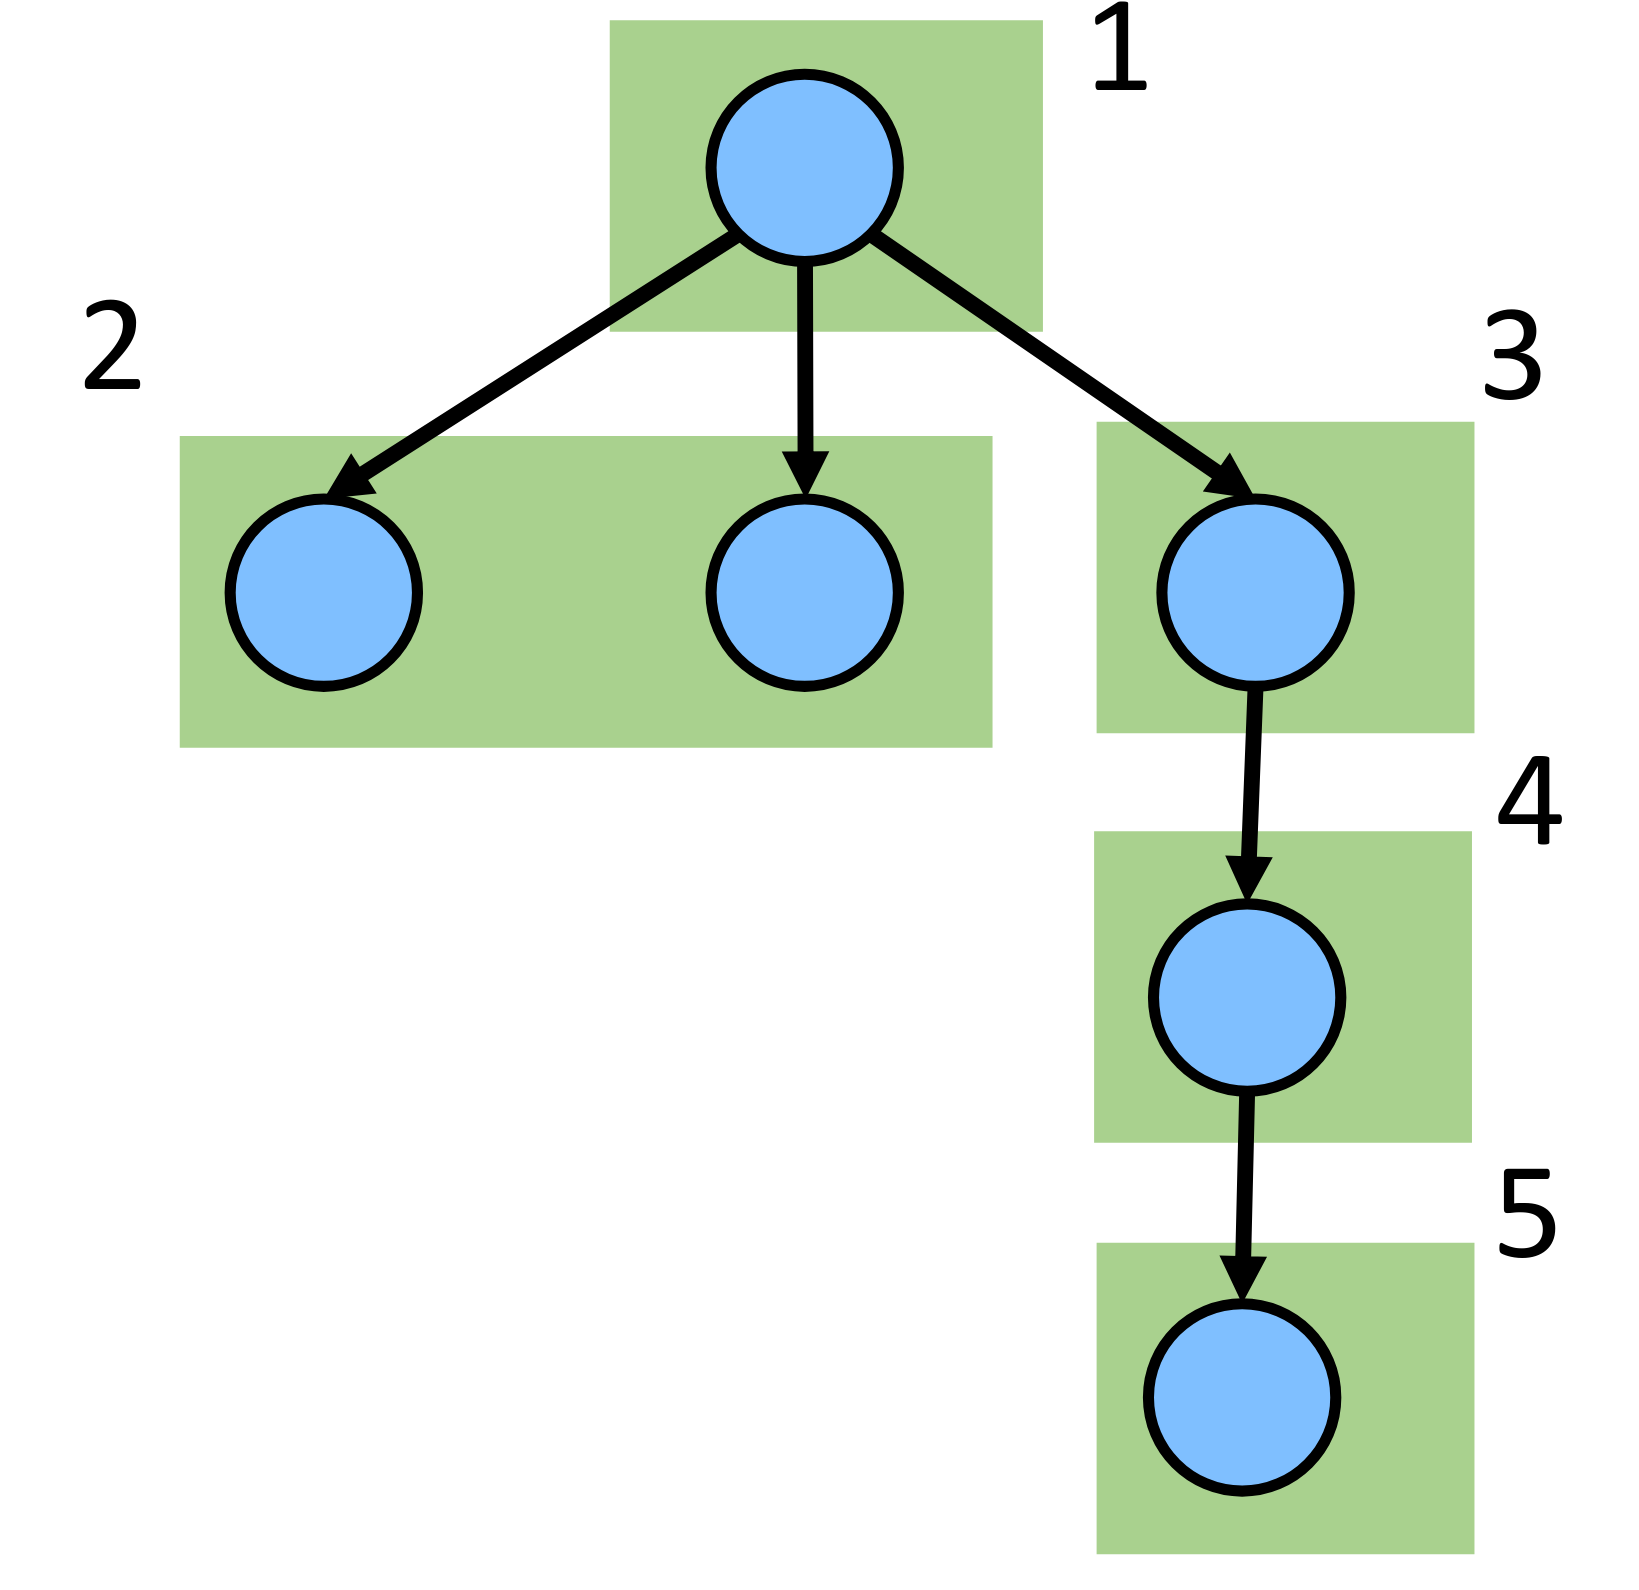
\includegraphics[scale=0.1]{Schedule1.png}
    \end{subfigure}
    \begin{subfigure}[t]{.5\textwidth}
        \centering
        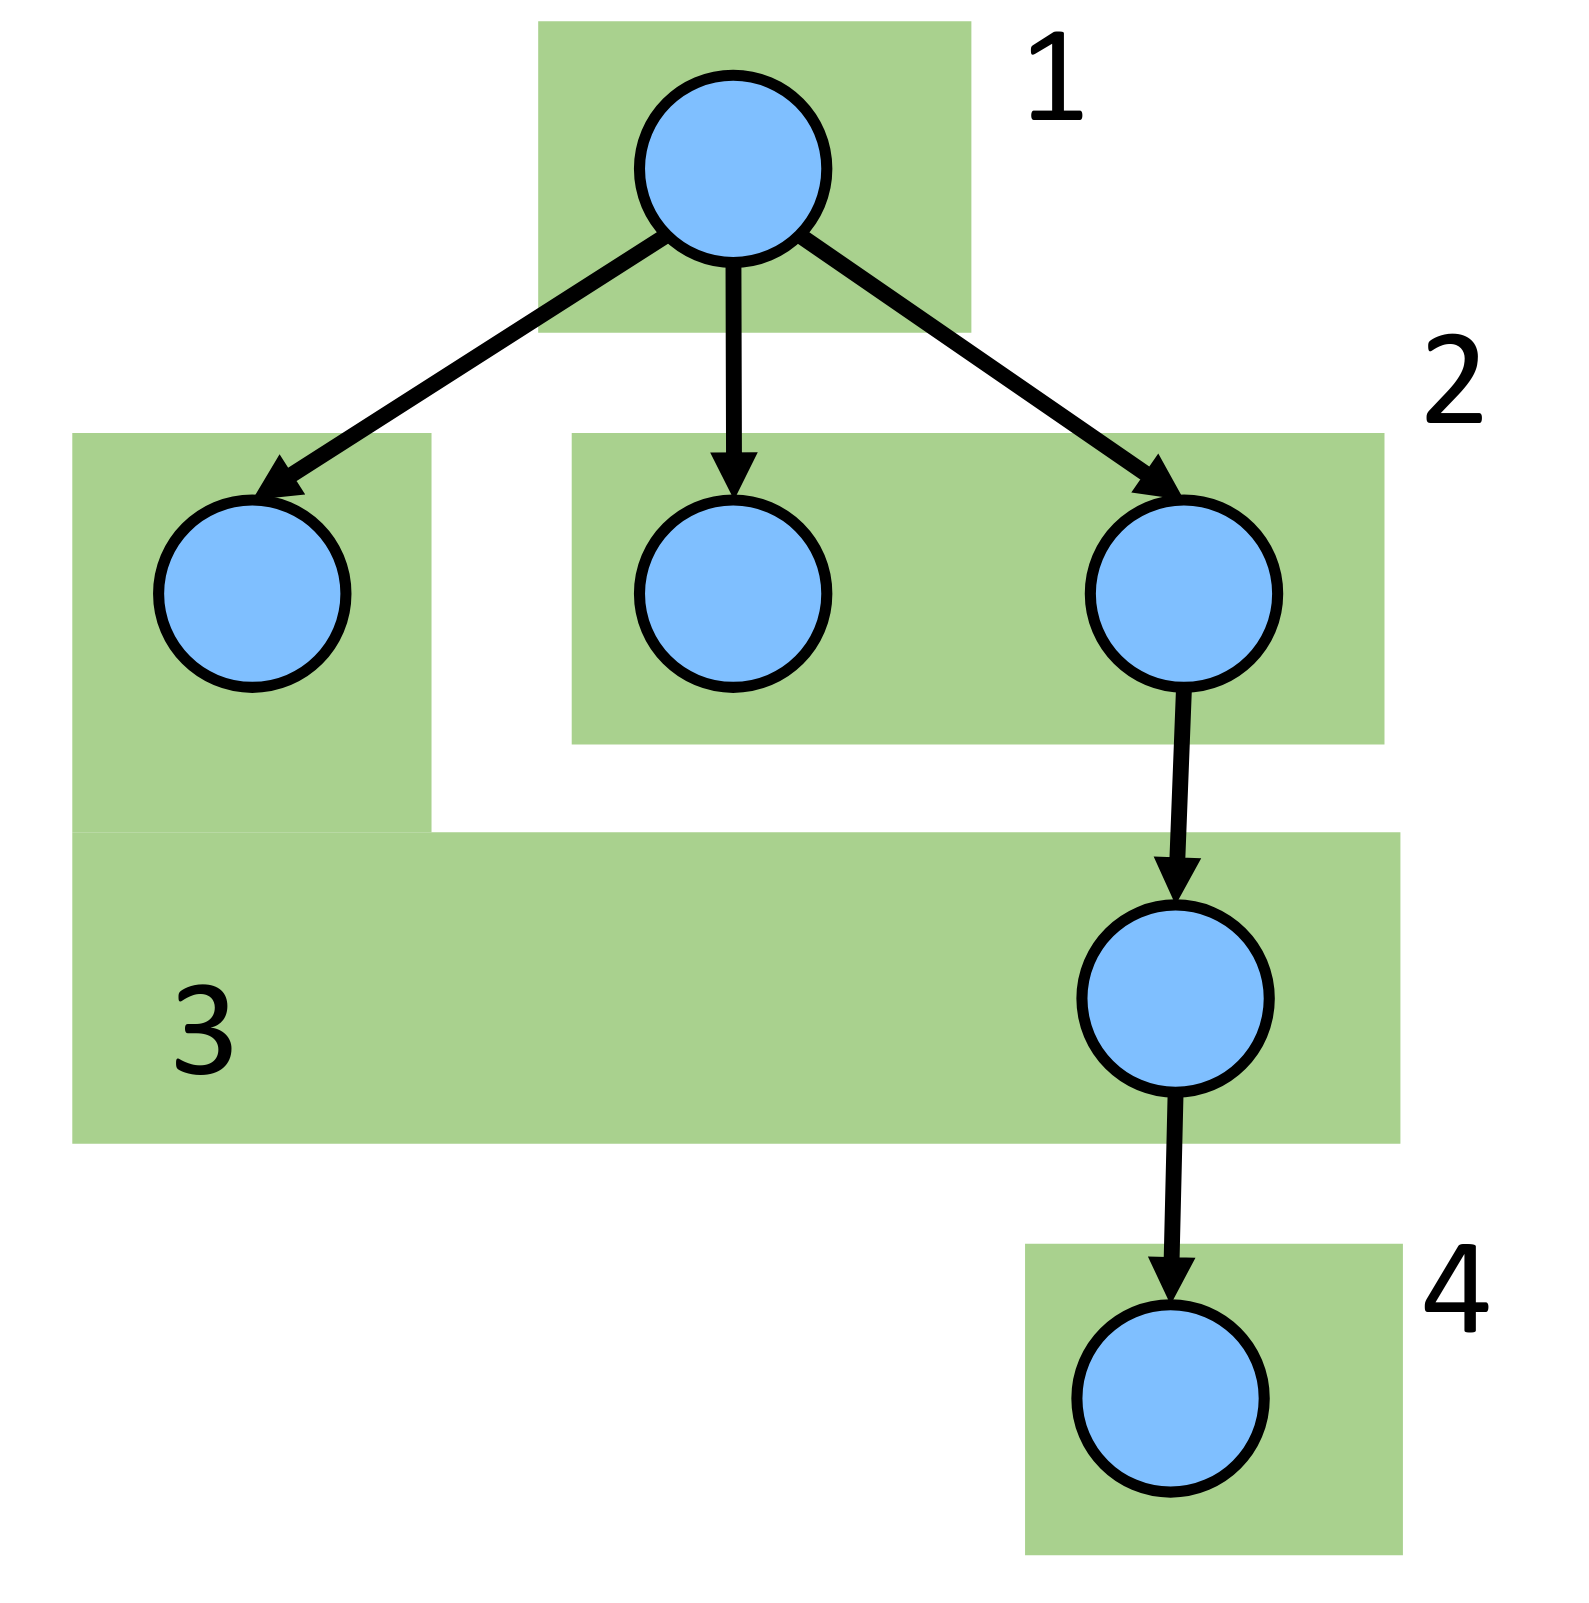
\includegraphics[scale=0.1]{Schedule2.png}
    \end{subfigure}
\end{figure}

\noindent In the first case, we can only exploit the second processor in the second time step. With this scheduling, \(T_{2}=5\). However, with the second scheduling, \(T_{2}=4\), which is optimal according to the span law.

\subsubsubsection{Runtime Guarantees of Cilk}
To get back to the subject matter, why did we introduce task graphs in this part of the course? Cilk introduced its task graph model in order to be able to prove theorems and thus provide guarantees about the execution of its programs.\\
In the previous section, we learned that \(T_{P}\) depends on the scheduling. A core of the Cilk language is its work-stealing scheduler that can provide strong runtime guarantees that are provable within this task graph model. In particular, Cilk gives us the following guarantee about the execution time on P processors:
$$\mathbb{E}(T_{P})=\mathcal{O}(\frac{T_{1}}{P} + T_{\infty})$$
\noindent That is, the expected time required to execute a Cilk program on P processors is equal to the critical path length \(T_{\infty}\) plus the sequential time \(T_{1}\) divided by the number of processors P. This is a strong guarantee, as both \(T_{\infty}\) and \(\frac{T_{1}}{P}\) are lower bounds on any parallel execution (span law and work law).\\
This means that a Cilk program has an expected runtime that is within a constant factor of optimal. The guarantee can only be given with regards to the expected value (and not about worst-case), because the work-stealing algorithm employs some randomization (for example randomizing which thread to steal work from). Of course we know that the O-notation can hide enormous constants. However, empirical testing showed that the runtime of Cilk programs is very close to optimal with small constants, that is, \(T_{p}\approx \frac{T_{1}}{P}+T_{\infty}\).\\
The important part for us in this course is that the Java Fork/Join framework is based on Cilk, adopting both its spawning/joining programming style and its work-stealing scheduler, thus also inheriting this strong runtime guarantee.

\subsubsection{Summary: Fork/Join Programming in Java}
After an odyssey where we...
\begin{enumerate}
  \item Recognized the \textbf{value of Fork/Join} patterns due to the simple program structure, ability to easily implement effective load balancing and parallelizing even the result combination.
  \item Recognized that using \textbf{Java threads for Fork/Join is not optimal}, since they block resources (memory, OS threads) and bring a lot of overhead (bookkeeping, context switching). To solve all these problems, we stumbled upon the \textbf{ExecutorService} framework, that offers light-weight tasks instead of heavy-weight threads. We had to notice that they are not designed for recursion.
  \item Found that the \textbf{Java Fork/Join framework} is exactly what we were looking for and enables us to reap all the benefits we originally hoped for from implementing parallel divide-and-conquer.
  \item Learned how the \textbf{Cilk programming language} pioneered multi-threading in programming languages and contributed a work-stealing scheduler enabling efficient Fork/Join parallelism that inspired Java to adopt most of its features within the Fork/Join framework. We learned that by modelling programs with task graphs, Cilk manages to prove asymptotic lower bounds on execution time that thus also apply to the Java Fork/Join framework.
\end{enumerate}
... we can now put Fork/Join in our toolbox for designing parallel algorithms and know how to effectively implement such algorithms in Java.

\subsection{Pack Pattern}


\subsection{Case Study: Parallelizing QuickSort}

\end{document}
